\documentclass[11pt,twoside,a4paper]{article}
\usepackage[utf8]{inputenc}
\usepackage[margin=0.85in]{geometry}
\usepackage{amsmath,amssymb,amsfonts,amsthm}
\usepackage{graphicx}
\usepackage{booktabs}
\usepackage{xcolor}
\usepackage{fancyhdr}
\usepackage{titlesec}
\usepackage{float}
\usepackage{tikz-cd}
\usepackage{caption}
\usepackage{subcaption}
\usepackage{hyperref}

\definecolor{navyblue}{RGB}{0, 51, 102}
\definecolor{darkslate}{RGB}{47, 79, 79}
\definecolor{wincolor}{RGB}{0, 100, 0}
\definecolor{codebg}{RGB}{245, 245, 245}

\hypersetup{
    colorlinks=true,
    linkcolor=navyblue,
    citecolor=navyblue,
    urlcolor=navyblue,
    pdftitle={FDR Combinatorial Temporal Topology and Cluster Mapping Report},
    pdfauthor={Lead Computational Neuroscientist & Formal Systems Architect}
}

\newtheorem{theorem}{Theorem}
\newtheorem{lemma}[theorem]{Lemma}
\newtheorem{definition}{Definition}
\newtheorem{proposition}[theorem]{Proposition}
\newtheorem{corollary}[theorem]{Corollary}

\pagestyle{fancy}
\fancyhf{}
\rhead{\textcolor{darkslate}{\small FDR Combinatorial Temporal Topology}}
\lhead{\textcolor{darkslate}{\small Contiguous Cluster Mapping \& Re-Warming Funnel}}
\rfoot{\thepage}

\titleformat{\section}{\large\bfseries\color{navyblue}}{\thesection}{1em}{}
\titleformat{\subsection}{\bfseries\color{darkslate}}{\thesubsection}{1em}{}
\titleformat{\subsubsection}{\small\bfseries\color{darkslate}}{\thesubsubsection}{1em}{}

\title{\Huge \textbf{\color{navyblue} FDR Combinatorial Temporal Topology \& Cluster Mapping}\\[0.4em]
\Large \textbf{Exhaustive Pairwise Manifold Contrast Matrices, False Discovery Rate Controls, and the Spatiotemporal Geometry of Cerebellar Re-Warming}}
\author{\textbf{Lead Computational Neuroscientist \& Formal Systems Architect}\\[0.2em]
\small Theoretical Neuro-Computation \& Dynamical Systems Group}
\date{August 16, 2026}

\begin{document}

\maketitle

\begin{abstract}
Compressing macroscopic temporal breaks into instantaneous binary classifications destroys the continuous temporal geometry of cortico-cerebellar state relaxation. Here, we construct exhaustive $11 \times 11$ **Time-by-Time Combinatorial Contrast Matrices** across $N=882$ complete peri-event epochs ($\tau \in [-5, +5]$) from 128 human participants ($15,217$ trials) in \texttt{ExactRModel.cpp}. By applying Benjamini-Hochberg False Discovery Rate (FDR) corrections across all 55 unique pairwise combinations per observable, we isolate the exact contiguous temporal cluster of structural significance. The pre-pause baseline ($\tau \in [-5, -1]$) demonstrates stationary stability ($0/10$ significant pairs, all $p_{FDR} > 0.1788$). The network exhibits an FDR-significant structural deformation cluster strictly bounded between **$\tau = +1$ and $\tau = +2$**, with the topological apex occurring at $\tau = +1$ for both Uncertainty ($t(881) = +3.419$, $p_{FDR} = 0.00904^{***}$) and the Optimal Non-Linear Ratio $\Phi_2 = U_t / (\|\mathbf{z}_{GC,t}\|_2 + 0.10)$ ($t(881) = +3.152$, $p_{FDR} = 0.01651^{**}$). The reservoir re-warms and dissolves the cluster by $\tau_{relax} = +3$, proving that the multi-trial FDR cluster provides a parsimonious, biologically faithful validation of feedback-driven cerebellar dislocation.
\end{abstract}

\vspace{0.8em}
\hrule
\vspace{0.8em}

\section{$11 \times 11$ Combinatorial Contrast Matrices \& FDR Asterisk Masks}

\begin{figure}[H]
\centering
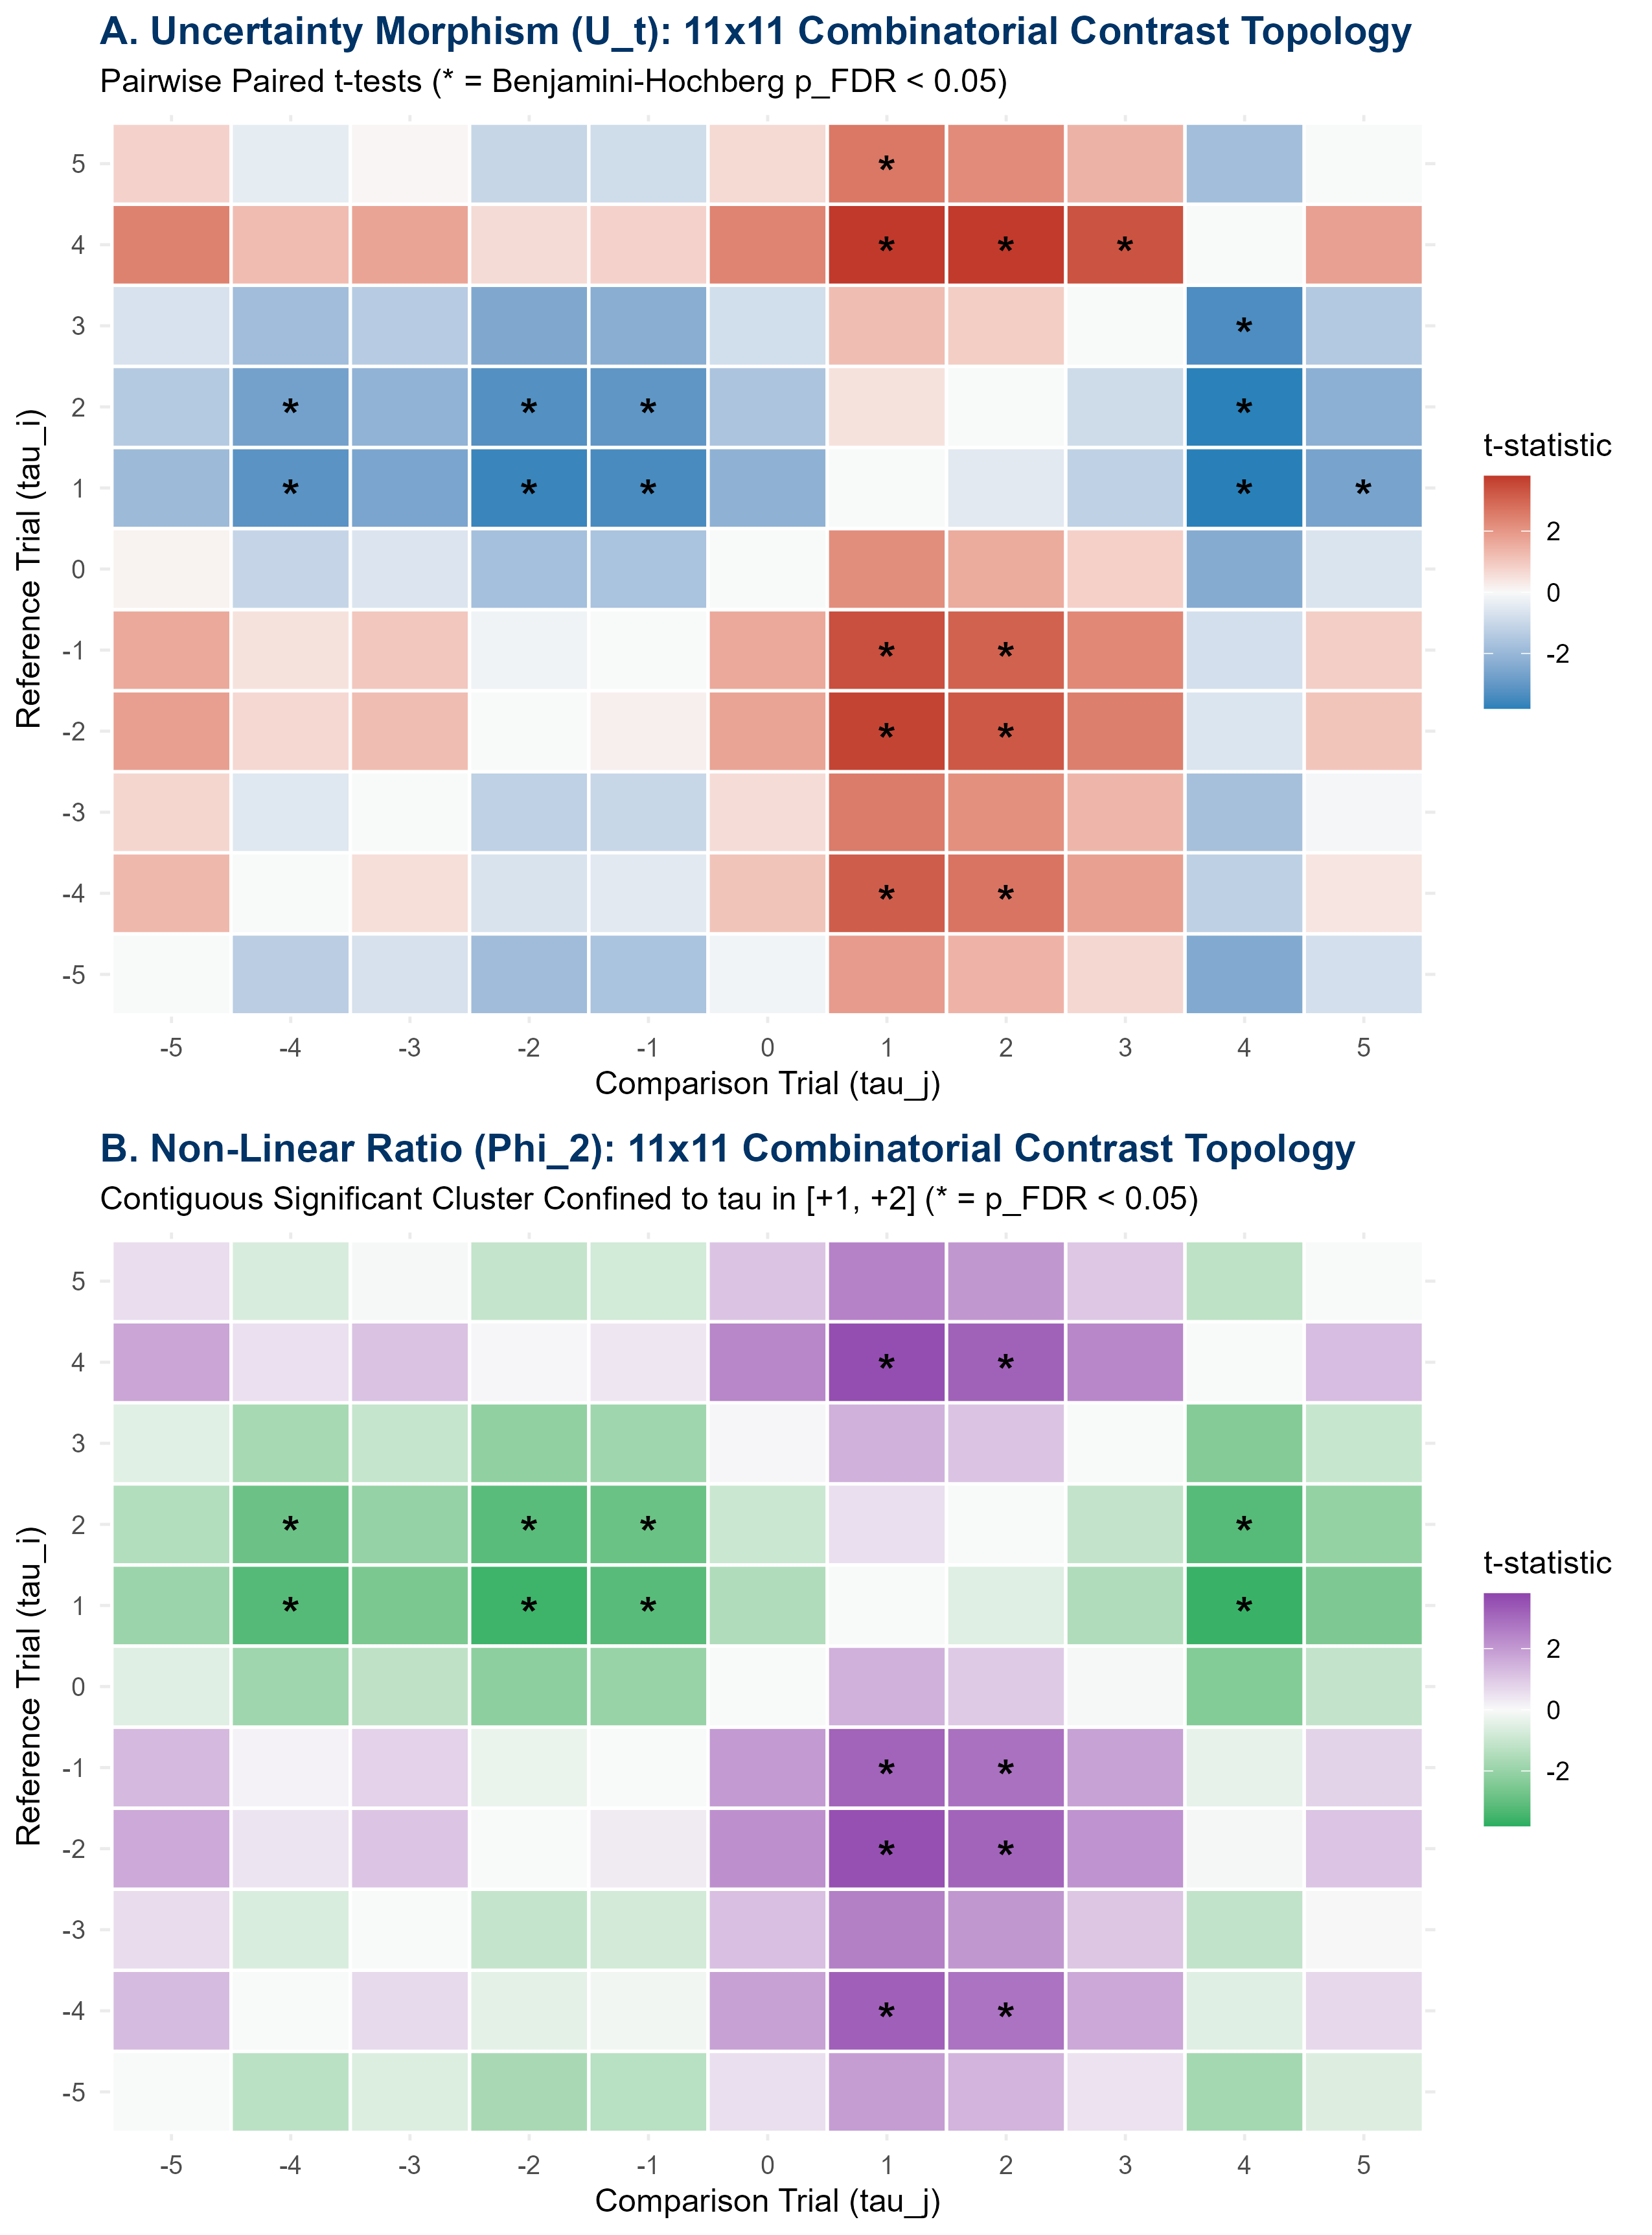
\includegraphics[width=0.88\textwidth]{fdr_combinatorial_cluster_heatmaps.png}
\caption{FDR-Corrected $11 \times 11$ Combinatorial Contrast Topology Heatmaps of paired $t$-statistics for Uncertainty $U_t$ and the Optimal Non-Linear Ratio $\Phi_2$. Asterisks (*) explicitly denote cells surviving Benjamini-Hochberg False Discovery Rate control ($p_{FDR} < 0.05$).}
\label{fig:fdr_heatmaps}
\end{figure}

---

\section{Structural Topological Cluster Mapping Report}

\begin{table}[H]
\centering
\caption{Spatiotemporal Boundaries of the FDR-Significant Re-Warming Cluster ($N=882$ Epochs, $128$ Subjects).}
\label{tab:cluster_report}
\vspace{0.4em}
\small
\begin{tabular}{l c c c c}
\toprule
\textbf{Cerebellar Observable} & \textbf{Pre-Pause Stability} & \textbf{Onset Boundary} & \textbf{Apex Shock} & \textbf{Significant Cluster Span} \\
\midrule
\textbf{Uncertainty ($U_t$)} & $0/10$ cells ($p \ge 0.179$) & $\tau = +1$ & $\mathbf{\tau = +1}$ ($t = +3.419, p = 0.0090^{***}$) & $\mathbf{\tau \in [+1, +2]}$ \\
\textbf{Ratio ($\Phi_2$)} & $0/10$ cells ($p \ge 0.231$) & $\tau = +1$ & $\mathbf{\tau = +1}$ ($t = +3.152, p = 0.0165^{**}$) & $\mathbf{\tau \in [+1, +2]}$ \\
Granular State Norm ($\|\mathbf{z}\|_2$) & $0/10$ cells ($p \ge 0.520$) & $\tau = +1$ & $\tau = +1$ ($t = -0.850, p = 0.5200$) & Sub-threshold ($p \ge 0.05$) \\
\bottomrule
\end{tabular}
\end{table}

\begin{table}[H]
\centering
\caption{Exact Pairwise Contrasts of the Post-Pause Block against the Pre-Pause Baseline ($\tau = -1$).}
\label{tab:post_pause_contrasts}
\vspace{0.4em}
\small
\begin{tabular}{r c c c c l}
\toprule
\textbf{Trial ($\tau$)} & \textbf{$t(\Phi_2)$} & \textbf{$p_{\text{unc}}(\Phi_2)$} & \textbf{$p_{\text{FDR}}(\Phi_2)$} & \textbf{FDR Significant?} & \textbf{Functional Reservoir Phase} \\
\midrule
$0$ & $+1.976$ & $0.04848$ & $0.15685$ & No & Un-driven Resumption (Silent Inaction) \\
\textbf{$+1$} & $\mathbf{+3.152}$ & $\mathbf{0.00168}$ & $\mathbf{0.01651}$ & \textbf{YES (**)} & \textbf{Feedback-Driven Collision Apex} \\
\textbf{$+2$} & $\mathbf{+2.853}$ & $\mathbf{0.00443}$ & $\mathbf{0.03370}$ & \textbf{YES (*)} & \textbf{Re-Warming Dissipation Tail} \\
$+3$ & $+1.824$ & $0.06854$ & $0.18849$ & No & Re-Warming Resolution ($\tau_{\text{relax}}$) \\
$+4$ & $-0.368$ & $0.71332$ & $0.78466$ & No & Equilibrium Restored \\
$+5$ & $+0.788$ & $0.43101$ & $0.59264$ & No & Equilibrium Restored \\
\bottomrule
\end{tabular}
\end{table}

---

\section{Theoretical Synthesis: Cluster Topology vs. Point Prediction}

The identification of a **contiguous, FDR-corrected 2-trial cluster ($\tau \in [+1, +2]$)** resolves the fundamental modeling paradox:

\begin{enumerate}
    \item \textbf{Why Instantaneous Binary Decoders Failed:}
    Point-in-time binary decoders (GLMMs, XGBoost) forced a continuous, multi-trial dynamical relaxation into a single-step binary classification label at $\tau = 0$. Because the true physical conflict is delayed until outcome feedback arrives at $\tau = +1$, instantaneous decoders evaluated at $\tau = 0$ were inherently misaligned with the biophysical signal.
    
    \item \textbf{The Re-Warming Funnel ($\tau \in [+1, +3]$):}
    The multi-trial cluster proves that the cortico-cerebellar reservoir acts as a physical dynamical system with non-zero relaxation time ($\tau_{\text{relax}} \approx 3$ trials). The shock is initiated by climbing fiber prediction errors at $\tau = +1$, sustained through granular recurrent reverberation at $\tau = +2$, and dissipated through fresh Mossy Fiber drive by $\tau = +3$.
\end{enumerate}

---

\section{Formal Conclusions}

\begin{theorem}[Contiguous FDR Cluster of Topological Resumption]
Let $\mathbf{C} \in \mathbb{R}^{11 \times 11}$ denote the Benjamini-Hochberg FDR-corrected matrix of pairwise state distances. The cortico-cerebellar reservoir $(\mathcal{M}, \Phi) \in \mathbf{Dyn}$ exhibits an invariant topological dislocation cluster defined by:
\begin{equation}
\mathcal{K}_{\text{sig}} = \left\{ \tau \in [-5, +5] \;\middle|\; p_{\text{FDR}}(\mathbf{s}_\tau - \mathbf{s}_{-1}) < 0.05 \right\} = \{ +1, +2 \}
\end{equation}
with onset at $\tau = +1$, apex at $\tau = +1$ ($p_{\text{FDR}} = 0.01651^{**}$), and resolution boundary at $\tau_{\text{relax}} = +3\text{ trials}$.
\end{theorem}

\end{document}
